\documentclass{fancydocument}

\usepackage{enumerate}
\usepackage{listings}
\usepackage{courier}
\usepackage{tabularx}
\usepackage{array}
\usepackage{graphicx}
\usepackage[all]{hypcap}
\usepackage{capt-of}

\title{Programmiersprachen benchmarken}
\title{Programmiersprachen benchmarken - \\ \renewcommand{\baselinestretch}{1.50}\large Programmiersprache ist nicht gleich Programmiersprache}
\author{Nick Zbinden und Matthias Gasser}
\date{\today}
\begin{document}
\maketitle
\thispagestyle{fancy}
\vspace*{\fill}
\noindent
Berufsbildungszentrum Bau und Gewerbe, Luzern\\
Klasse: BML08E
\newpage
\tableofcontents
\definecolor{lineno}{rgb}{0.5,0.5,0.5}
\definecolor{code}{rgb}{0,0.1,0.6}
\definecolor{keyword}{rgb}{0.5,0.1,0.1}
\definecolor{titlebox}{rgb}{0.85,0.85,0.85}
\definecolor{download}{rgb}{0.8,0.1,0.5}
\definecolor{title}{rgb}{0.4,0.4,0.4}

\lstdefinelanguage{Clojure}
{
    morekeywords={*agent*, *clojure-version*, *command-line-args*, *compile-files*, *compile-path*, *e, *err*, *file*, *flush-on-newline*, *in*, *ns*, *out*, *print-dup*, *print-length*, *print-level*, *print-meta*, *print-readably*, *read-eval*, *warn-on-reflection*, +, -, ->, ->>, .., /, <, <=, =, ==, >, >=, accessor, aclone, add-classpath, add-watch, agent, agent-error, agent-errors, aget, alength, alias, all-ns, alter, alter-meta!, alter-var-root, amap, ancestors, and, apply, areduce, array-map, aset, aset-boolean, aset-byte, aset-char, aset-double, aset-float, aset-int, aset-long, aset-short, assert, assoc, assoc!, assoc-in, associative?, atom, await, await-for, bases, bean, bigdec, bigint, binding, bit-and, bit-and-not, bit-clear, bit-flip, bit-not, bit-or, bit-set, bit-shift-left, bit-shift-right, bit-test, bit-xor, boolean, boolean-array, booleans, bound-fn, bound-fn*, bound?, butlast, byte, byte-array, bytes, case, cast, char, char-array, char-escape-string, char-name-string, char?, chars, class, class?, clear-agent-errors, clojure-version, coll?, comment, commute, comp, comparator, compare, compare-and-set!, compile, complement, concat, cond, condp, conj, conj!, cons, constantly, construct-proxy, contains?, count, counted?, create-ns, create-struct, cycle, dec, decimal?, declare, definline, defmacro, defmethod, defmulti, defn, defn-,def, defonce, defprotocol, defrecord, defstruct, deftype, delay, delay?, deliver, denominator, deref, derive, descendants, disj, disj!, dissoc, dissoc!, distinct, distinct?, doall, doc, dorun, doseq, dosync, dotimes, doto, double, double-array, doubles, drop, drop-last, drop-while, empty, empty?, ensure, enumeration-seq, error-handler, error-mode, eval, even?, every?, extend, extend-protocol, extend-type, extenders, extends?, false?, ffirst, file-seq, filter, find, find-doc, find-ns, find-var, first, flatten, float, float-array, float?, floats, flush, fn, fn?, fnext, fnil, for, force, format, frequencies, future, future-call, future-cancel, future-cancelled?, future-done?, future?, gen-class, gen-interface, gensym, get, get-in, get-method, get-proxy-class, get-thread-bindings, get-validator, group-by, hash, hash-map, hash-set, identical?, identity, if-let, if-not, ifn?, import, in-ns, inc, init-proxy, instance?, int, int-array, integer?, interleave, intern, interpose, into, into-array, ints, io!, isa?, iterate, iterator-seq, juxt, keep, keep-indexed, key, keys, keyword, keyword?, last, lazy-cat, lazy-seq, let, letfn, line-seq, list, list*, list?, load, load-file, load-reader, load-string, loaded-libs, locking, long, long-array, longs, loop, macroexpand, macroexpand-1, make-array, make-hierarchy, map, map-indexed, map?, mapcat, max, max-key, memfn, memoize, merge, merge-with, meta, methods, min, min-key, mod, name, namespace, namespace-munge, neg?, newline, next, nfirst, nil?, nnext, not, not-any?, not-empty, not-every?, not=, ns, ns-aliases, ns-imports, ns-interns, ns-map, ns-name, ns-publics, ns-refers, ns-resolve, ns-unalias, ns-unmap, nth, nthnext, num, number?, numerator, object-array, odd?, or, parents, partial, partition, partition-all, partition-by, pcalls, peek, persistent!, pmap, pop, pop!, pop-thread-bindings, pos?, pr, pr-str, prefer-method, prefers, print, print-namespace-doc, print-str, printf, println, println-str, prn, prn-str, promise, proxy, proxy-mappings, proxy-super, push-thread-bindings, pvalues, quot, rand, rand-int, rand-nth, range, ratio?, rationalize, re-find, re-groups, re-matcher, re-matches, re-pattern, re-seq, read, read-line, read-string, reduce, reductions, ref, ref-history-count, ref-max-history, ref-min-history, ref-set, refer, refer-clojure, reify, release-pending-sends, rem, remove, remove-all-methods, remove-method, remove-ns, remove-watch, repeat, repeatedly, replace, replicate, require, reset!, reset-meta!, resolve, rest, restart-agent, resultset-seq, reverse, reversible?, rseq, rsubseq, satisfies?, second, select-keys, send, send-off, seq, seq?, seque, sequence, sequential?, set, set-error-handler!, set-error-mode!, set-validator!, set?, short, short-array, shorts, shuffle, shutdown-agents, slurp, some, sort, sort-by, sorted-map, sorted-map-by, sorted-set, sorted-set-by, sorted?, special-form-anchor, special-symbol?, spit, split-at, split-with, str, string?, struct, struct-map, subs, subseq, subvec, supers, swap!, symbol, symbol?, sync, syntax-symbol-anchor, take, take-last, take-nth, take-while, test, the-ns, thread-bound?, time, to-array, to-array-2d, trampoline, transient, tree-seq, true?, type, unchecked-add, unchecked-dec, unchecked-divide, unchecked-inc, unchecked-multiply, unchecked-negate, unchecked-remainder, unchecked-subtract, underive, update-in, update-proxy, use, val, vals, var-get, var-set, var?, vary-meta, vec, vector, vector-of, vector?, when, when-first, when-let, when-not, while, with-bindings, with-bindings*, with-in-str, with-local-vars, with-meta, with-open, with-out-str, with-precision, xml-seq, zero?, zipmap, recur},
   sensitive,
   alsodigit=-,
   morecomment=[l];,
   morestring=[b]"
  }[keywords,comments,strings]

% "define" Scala
\lstdefinelanguage{scala}{
  morekeywords={abstract,case,catch,class,def,%
    do,else,extends,false,final,finally,%
    for,if,implicit,import,match,mixin,%
    new,null,object,override,package,%
    private,protected,requires,return,sealed,%
    super,this,throw,trait,true,try,%
    type,val,var,while,with,yield},
  otherkeywords={=>,<-,<\%,<:,>:,\#,@},
  sensitive=true,
  morecomment=[l]{//},
  morecomment=[n]{/*}{*/},
  morestring=[b]",
  morestring=[b]',
  morestring=[b]"""
}

\lstset{
         language=Clojure,
         basicstyle=\footnotesize\ttfamily, % Standardschrift
         %numbers=left,               % Ort der Zeilennummern
         numberstyle=\tiny,          % Stil der Zeilennummern
         %stepnumber=2,               % Abstand zwischen den Zeilennummern
         numbersep=5pt,              % Abstand der Nummern zum Text
         tabsize=2,                  % Groesse von Tabs
         extendedchars=true,         %
         breaklines=true,            % Zeilen werden Umgebrochen
         keywordstyle=\color{red},         
         stringstyle=\color{black}\ttfamily, % Farbe der String
         showspaces=false,           % Leerzeichen anzeigen ?
         showtabs=false,             % Tabs anzeigen ?
         xleftmargin=17pt,
         framexleftmargin=17pt,
         framexrightmargin=5pt,
         framexbottommargin=4pt,
         showstringspaces=false      % Leerzeichen in Strings anzeigen ?        
}

\newcolumntype{v}[1]{%
  >{\raggedright\hspace{0pt}\arraybackslash}p{#1}%
}
\newpage
\section{Vorwort}

Die Informatik hat auf uns schon immer eine gewisse Faszination ausgeübt. Es war daher für uns beide naheliegend eine Lehre als Informatiker zu machen. Während Nick vor allem an der Softwareentwicklung interessiert ist, bevorzuge ich die Systemtechnik, in der die Installation und Wartung von IT-Systemen der Grosse Schwerpunkt ist.
Da wir beide unsere Berufe noch immer sehr interessiert ausführen, war es für uns beide klar für die IDPA ein Thema aus dem Bereich Informatik zu wählen. Es galt nun ein Thema zu finden, in dem sowohl die Applikationsentwicklung wie auch die Systemtechnik gleichermassen eine Rolle spielen. Bereits nach kurzer Recherche stiessen wir auf das Thema „Programmiersprachen Benchmarking“. Sofort war unser beider Interesse geweckt und dadurch,  dass dieses Thema sowohl ein Testsystem wie auch selbstgeschriebene Programme erforderte, eignete es sich sehr gut für eine IDPA. Wir entschieden uns, unsere Maturaarbeit diesem Thema zu widmen.

Am gewählten Thema interessiert uns beide in erster Linie ob tatsächlich Performanceunterschiede zwischen den untersuchten Sprachen feststellbar sind, und in welchem Ausmass sie sich zeigen. Heutige Computer sind sehr leistungsfähig, dadurch ist es für kleinere Programme wie wir sie testen werden meist irrelevant ob eine Programmiersprache einige Millisekunden schneller ist als die andere. Für grössere Projekte spielt die Geschwindigkeit jedoch auch heute noch eine wichtige Rolle, wir hoffen daher, dass sich unsere Testergebnisse auf grössere Applikationen projizieren lassen.

\section{Abstract}
Wir haben uns entschieden für unsere Maturaarbeit die Programmiersprachen Java, Clojure und Scala zu vergleichen. Wir haben dazu ein identisches Programm in jeder der genannten Programmiersprachen geschrieben. Durch das Messen von Prozessor- und Speicherdaten sowie der Ausführungszeiten der Programme wollten wir Unterschiede feststellen, um am Ende aufzeigen zu können, welche der getesteten Sprachen vom Testsystem am wenigsten Leistung abverlangt. Für die Messungen haben wir ein Script geschrieben, welches die erforderlichen Daten in angemessenen Zeitabständen ausliest. Nach Auswertung der gemessenen Daten zeigte sich, dass Clojure das System bei weitem am wenigsten belastet. Jedoch war die Ausführungszeit für das Clojure Programm ungefähr drei Mal so lange wie diejenige der anderen Sprachen. Da in der Programmierung heutzutage Geschwindigkeit wichtiger ist als alles andere, raten wir davon ab Clojure für grössere Projekte zu verwenden, da die sehr junge Sprache schlicht noch nicht genügend ausgereift ist. Scala und Java lieferten beide sehr ähnliche Resultate. Bei einer beinahe identischen Ausführungszeit benötigte Scala jedoch immer leicht weniger Systemressourcen als Java. Da Ressourcen bei aktuellen Computern meist jedoch kaum mehr eine Rolle spielen, sollte wenn immer möglich die schnellste Programmiersprache, d.h. Java, verwendet werden.
\section{Einleitung}

\subsection{Untersuchungsgegenstand}

Wir haben uns ein sehr komplexes Thema vorgenommen. Programmiersprachen und Compiler sind, auf die Informatik bezogen, einen sehr altes Thema. \\
Hochsprachen wie wir sie in dieser Arbeit verwenden, werden seit mehr
als fünfzig Jahren immer wieder weiter entwickelt und verbessert. Seit
der Anfangszeit herrscht der Konflikt zwischen hoher Abstraktion und
Geschwindigkeit. Umso höher die Abstraktion ist, die eine
Programmiersprache bietet, umso schwieriger ist die Programmiersprache
auf der darunterliegenden Sprache effizient auszuführen.


\subsection{Problemstellung}

Wir haben uns die Aufgabe gestellt drei Programmiersprachen unter dem
Aspekt der Geschwindigkeit anzuschauen und zu vergleichen. Eine
definitives Ergebnis ist in diesem Bereich fast unmöglich da die
Anwendungsgebiete einer Programmiersprache zu verschieden sind und
jeder Anwendungsfall andere Anforderungen hat. Auch die
unter der Programmiersprache liegenden Layer (Betriebssystem und
Hardware) sind von entscheidender Bedeutung. Um korrekte Aussagen zu
machen m\"ussen diese Layer entweder herausgerechnet werden oder
identisch sein. Das Ziel ist es f\"ur den von uns ausgew\"ahlten Anwendungsfall Messungen
zu machen, Aussagen \"uber die Geschwindigkeiten zu treffen und
wenn m\"oglich kl\"aren warum die Sprachen sich so verhalten.

\subsection{Wissenslücken}

Um komplizierte Algorithmen in drei verschiedenen Sprachen zu
programmieren braucht man viel Erfahrung in diesen Sprachen. Um den
Aufwand nicht zu hoch werden zu lassen haben wir uns auf die
Implementierung in einer Programmiersprache beschränkt und
vergleichen diese mit Referenz-Implementationen die wir nur erklären
und messen.

Um genau zu erkennen wo Programme ihre Zeit verbringen, benötigt man
komplexe Analyse Tools oder speziell dafür ausgelegte VMs. Diese Tools
sind komplex in der Verwendung und man braucht viel Erfahrung mit einem
System um aus den Information auch die richtigen Schlüsse ziehen zu können.

\subsection{Erwartungen}

Es ist das erkl\"arte Ziel von Clojure und
Scala genauso schnell zu sein wie Java, damit der Programmierer niemals aus Geschwindigkeitsgründen auf Java zurückgreifen muss. Wir haben daher die Hypothese aufgestellt, dass es für Scala relativ einfach ist
gleichschnellen Code wie Java zu produzieren, da beide Sprachen 
statische Typeninformation haben. Ausserdem ist Scala Java sehr ähnlich
und Scala ist eine der \"altesten und reifsten JVM-Sprachen.

Die Erwartungen an Clojure sind nicht ganz so hoch da das Clojure-Projekt relativ neu ist. Clojure 
ist ausserdem eine dynamische Programmiersprache, diese sind schwerer zu optimieren.


\section{Material und Methoden}

\subsection{Allgemeines}

\subsubsection{Sprachauswahl}

In den letzten Jahren ist ein neuer Trend
entstanden. Programmiersprachen werden oft nicht mehr von Grund auf neu
aufgebaut sondern versuchen bestehende Infrastrukturen zu verwenden.
\\
Dies bringt sowohl Vor- als auch Nachteile mit sich. Hauptvorteil ist, dass
man sich als Trittbrettfahrer eine VM zunutze machen kann. In moderne
VMs, wie der JVM, wurden hunderte von Mannjahren investiert. Sie sind
daher sehr stabil und auf vielen Computern bereits installiert.

Der zweite Vorteil ist die Interoperabilität zwischen den
verschiedenen Sprachen. Dadurch kann Code
wiederverwendet werden ohne dass viel Zeit in die Portierung von
Funktionen investiert werden muss welche jede Sprache braucht. Dies können beispielsweise Datenbanken, Protokolle oder XML Parser sein. In der Java Programmiersprache sind all diese grundlegenden Funktionen
bereits implementiert. Die JVM ist daher eine geeignete Plattform um andere
Sprachen darauf aufzusetzen.

Die entscheidende Frage ist nun weshalb die Nutzer die neuen
Sprachen ben\"utzen sollten. Dafür gibt es viele Gründe. Einige neue
Sprachen (Scala) bieten bessere Typsysteme und dadurch mehr
Compiletime Sicherheiten. Andere Sprachen, wie z.B. Groovy, versuchen Features
von sehr dynamischen Sprachen zu unterst\"utzen.

Alle diese neuen und spannenden Features sind fantastisch, gehen aber
oft zu Lasten der Performance. Das kommt teilweise davon, dass manche Features (z.B. Bouncechecking)
bereits per Definition performancelastig sind, oft stellt jedoch auch der Unterschied in den Semantiken der Sprachen ein Problem dar. D.h. wenn in einer Sprache ein Feature
unterst\"utzt wird in der Host-VM jedoch nicht, muss um das Problem herum
gearbeitet werden was zus\"atzlichen Runtime-Overhead verursacht. In dieser
Arbeit haben wir uns zwei der meist verwendeten neuen JVM-Sprachen
ausgesucht um herauszufinden ob diese es schaffen die Geschwindigkeit
der Hostsprache (Java) zu erreichen.

\subsubsection{Zielanpassung: Sprachanpassung}

Gemäss Exposé wollten wir die drei JVM-Sprachen Clojure, Scala und JRuby
Benchmarken. W\"ahrend der Arbeit haben wir
festgestellt, dass JRuby andere Ziele verfolgt als maximale
Performance zu bieten und es deshalb weder produktiv noch sinnvoll ist
JRuby mit Clojure und Scala, die beide diesen Anspruch haben, zu
vergleichen.

Um JRuby zu ersetzen h\"atten wir eine weitere neue JVM-Sprache
wählen k\"onnen (es gibt mehr als einhundert), es gibt jedoch kaum andere
Sprachen die weit genug entwickelt sind oder die \"ahnliche Ziele
verfolgen. Deshalb haben wir uns Entschieden zu testen, ob
Clojure und Scala wirklich die Geschwindigkeit von Java erreichen.

\subsubsection{Zielanpassung: Implementierung}

Anfangs hatten wir geplant einen Algorithmus in drei verschiedenen Sprachen zu
implementieren und dann die Performance zu messen. Um einen mehr oder
weniger komplexen Algorithmus in drei Sprachen zu implementieren muss
man diese Sprachen sehr gut kennen und verstehen. Noch schwieriger
wird es wenn Performanceoptimierungen gefragt sind. Viele
Sprachen lassen sich extrem "verbiegen"  wodurch sich, auf Kosten von
Einfachheit und Klarheit, die Geschwindigkeit verbessern lässt.

Wir verfügen nicht über ausreichen Fachwissen um solche Programme zu schreiben und sich dieses
anzueignen erfordert eine monatelagen Einarbeitungszeit. Deshalb
beschr\"anken wir uns, bei der Implementierung, auf eine Sprache. Für
die anderen Tests benutzen wir Referenz-Implementierungen.

\subsection{Grundlagen}

\subsubsection{Virtuelle Maschinen}

Um es simpel zu halten haben wir uns entschieden
Programmiersprachen zu verwenden, die auf der JVM (oder anderen VMs die
Java Byte Code ausf\"uhren) laufen. Dies erlaubt uns Aussagen \"uber die
Codegenerierung des Source-to-Bytecode-Compilers der jeweiligen Sprachen
machen.
\\
Da VMs einen Bytecode als Input erhalten, ist es grunds\"atzlich m\"oglich
jede Programmiersprache auf einer VM laufen zu lassen. Wie dieser
Bytecode in der VM ausgef\"uhrt wird, ist den dar\"uber liegenden Sprachen
egal.\\ 

Einige Möglichkeiten wie eine VM den Bytecode ausführt:


\begin{itemize}
\item Interpreter
\item JIT-Compiler
\item Native Code Compiler
\item Direkt auf Hardware
\end{itemize}

Ich m\"ochte nur auf den JIT-Compiler etwas n\"aher eingehen da die JVM,
die wir ben\"utzen, einen solchen verwendet (Hotspot). Um zu verstehen warum ein
Programm langsam oder schnell ist muss man bis zu einem gewissen Grad
den Compiler verstehen.

\subsubsection{JIT-Compiler}

Ein JIT-Compiler kompiliert nicht alles auf einmal sondern, nur den
Code der auch wirklich gebraucht wird. Das erlaubt dem Compiler
Optimierungen an den wichtigen Stellen anzubringen. Ein weiterer
grosser Vorteil ist es, dass dem JIT-Compiler die Umgebung auf der er
sich befindet bekannt ist. Das erlaubt es Optimierungen vorzunehmen,
die speziell für diese Hardware den Code anpassen.
\\
Gute JIT-Compiler sind heutzutage geschwindigkeitsmässig vergleichbar den Native Code Compilern. Die Unterschiede sind in vielen
Anwendungsf\"allen nur noch gering.

\subsection{Das Testsystem}
\subsubsection{Leistungsdaten}
Beim verwendeten Testsystem  handelt es sich um einen HP Compaq 6710b Notebook mit den folgenden Leistungsdaten.

\begin{itemize}
\item Prozessor: Intel Core 2 Duo T7700 @ 2.4 GHz
\item Arbeitsspeicher: 2 GB
\end{itemize}

Wir haben uns entschieden als Betriebssystem die aktuellste Version der Linux-Distribution Debian zu verwenden. Debian hat die Vorteile, dass es sehr stabil läuft und einfacher zu bedienen ist, als andere Linux-Distributionen. Wir haben uns aus verschiedenen Gründen dafür entschieden unsere Tests Linux-basierend durchzuführen. So ist unter Linux keine Lizenzierung nötig, da das Betriebssystem und der grösste Teil der Programme Open-Source sind  oder  wir haben durch vorgängige Recherchen festgestellt, dass die Auswahl an freien Performance-Monitoring-Tools in der Linux-Welt viel grösser ist.
Die genannten Leistungsdaten sind für die Nachvollziehbarkeit der Messdaten sehr wichtig. Werden die Tests auf einem anderen System wiederholt, kann nicht sichergestellt werden, dass die Resultate identisch sind. 
Des Weiteren ist zu erwähnen, dass obwohl der installierte Prozessor über zwei Cores verfügt, die Testprogramme nur darauf ausgelegt sind, einen zu nutzen. Eine Lastverteilung durch das Betriebssystem findet jedoch trotzdem statt. Die Hauptgründe dafür, dass nur ein Kern genutzt wird, sind die folgenden:

\begin{itemize}
\item Der Programmieraufwand ist kleiner, wenn nur ein Kern genutzt wird
\item Eine Parallelisierung lohnt sich bei zwei Kernen vielfach nicht da der zusätzliche Rechenaufwand grösser ist als der Geschwindigkeitsgewinn.
\end{itemize}

\subsubsection{Swap-Space}
Der Swap-Space ist ein virtueller Speicher welcher vom Betriebssystem genutzt wird, wenn der eingebaute Arbeitsspeicher nicht ausreicht. In der MS Windows-Welt ist der Swap-Space unter der Bezeichnung „Auslagerungsdatei“ bekannt. Der Swap-Space befindet sich auf der Festplatte und ist daher um ca. Faktor 1000 langsamer als der Arbeitsspeicher. Trotzdem ist es wichtig, dass das Betriebssystem notfalls in der Lage ist auf einen Swap zurückgreifen zu können. Ansonsten kann dies zu abstürzen von einzelnen Prozessen oder gar dem ganzen System führen. Da gerade die JVM relativ speicherintensiv ist, wird dies umso wichtiger.

Ein viel diskutiertes Thema wenn es um den Swap-Space geht, ist dessen Grösse. Grundsätzlich wird empfohlen den Swap-Space mindestens gleich gross wie den Arbeitsspeicher, aber höchstens doppelt so gross zu machen. Ich habe mich daher an die Faustregel Swap-Space = 1.5 * Arbeitsspeicher gehalten. Nach oben sind theoretisch übrigens keine Grenzen gesetzt, jedoch ist es fraglich ob ein System jemals einen noch grösseren Swap-Space auslasten wird. Es ist daher reine Speicherverschwendung grössere Bereiche auf der Festplatte für Swap zu reservieren.

\subsection{Aufnahme der Daten}
Nach gründlichen Recherchen und dem Testen diverser Monitoring-Tools kamen wir leider zu Schluss, dass kein Programm unsere Anforderungen ausreichend erfüllen konnte. Das Hauptproblem war meist, dass die Datenaufnahme nicht automatisch gestartet werden konnte. Die Aufzeichnung der Daten manuell zu starten, kam für uns jedoch nicht in Frage, da bereits eine Sekunde Verzögerung zwischen Programmstart und Start der Datenaufnahme den Verlust einer Grossen Datenmenge zur Folge hätte. Des Weiteren boten einige Programme keine oder  nur beschränkte Möglichkeiten um die gesammelten Daten zu speichern.

Als Alternative haben wir uns für ein selbstgeschriebenes Script entschieden. Linux bringt selbst bereits eine Vielzahl an Funktionen mit um Leistungsdaten auszulesen. Bereits nach kurzer Nachforschung zeigte sich, dass eine Automatisierung des Auslesevorgangs mittels Script relativ einfach zu realisieren ist.

\subsubsection{Das Script}
Das folgende Script liest die benötigten Leistungsdaten aus. Ich erkläre die einzelnen Bereiche des Scripts nacheinander um Verwirrung zu vermeiden.

Die erste Zeile informiert Linux darüber, dass es sich um ein Shell-Script handelt, damit das Betriebssystem den Code richtig interpretieren kann. Bei einem Perl Script müsste hier beispielsweise das ‚sh‘ durch ein ‚perl‘ ersetzt werden.

\begin{minipage}{\textwidth}
\begin{lstlisting}[language=bash,caption=Shebang]{}
#!/bin/sh
\end{lstlisting}
\end{minipage}
Die als Parameter mitgegebenen Parameter werden in Variablen gespeichert.

\begin{minipage}{\textwidth}
\begin{lstlisting}[language=bash,caption=Parameter]{}
lang=$1
code=$2
param=$3
\end{lstlisting}
\end{minipage}

Nun folgt die Fehlerbehandlung.  Die erste Zeile besagt, dass wenn im Script ein Fehler auftritt, welcher nicht zuvor durch eine andere Funktion abgefangen wird, die Funktion „error“ ausgeführt werden soll. Dabei ist es egal wodurch der Fehler verursacht wird oder an welcher Stelle er auftritt.

Die Error-Funktion gibt ihrerseits eine Meldung aus, die den Benutzer über das Auftreten des Fehlers aufklärt und evtl. mögliche Ursachen dafür nennt. Anschliessend wird das Script beendet.

\begin{minipage}{\textwidth}
\begin{lstlisting}[language=bash,caption=Fehlerbehandlung,literate=% 
{ü}{{\"u}}1 
{ä}{{\"a}}1 
{ö}{{\"o}}1]{}
trap "error" ERR
#
function error() {
	echo '
##########
Ein unbekannter Fehler ist aufgetreten. Prüfen Sie die folgenden möglichen Fehlerquellen:
- ungültige Java Parameter
- fehlerhafte Programmdatei (*.jar)
##########'
	exit 0
}
\end{lstlisting}
\end{minipage}

Die folgenden beiden Vergleichsoperationen (IF-Konstrukte) dienen ebenfalls der Fehlerbehandlung. Die erste Funktion prüft ob die angegebene Sprache zulässig ist (wenn die Sprache im Parameter \$lang nicht Clojure ist und nicht Java ist und nicht Scala ist, dann führe den folgenden Code aus). Wenn der Vergleich wahr ist, d.h. eine falsche Sprache angegeben wurde, wird eine entsprechende Meldung ausgegeben und das Script beendet.

\begin{minipage}{\textwidth}
\begin{lstlisting}[language=bash,caption=Sprachparameter prüfen]{}
if [ $lang != clojure -a $lang != java -a $lang != scala ] ; then
	echo 'Enter clojure, java or scala for Parameter 1!'
	exit 0
fi
\end{lstlisting}
\end{minipage}

Die zweite Vergleichsoperation überprüft, ob die angegebene auszuführende Programmdatei überhaupt auffindbar ist (wenn die Datei im Parameter \$code nicht vorhanden ist, dann führe den folgenden Code aus). Sollte das Script keine Datei finden können, wird der Benutzer informiert und das Script beendet.

\begin{minipage}{\textwidth}
\begin{lstlisting}[language=bash,caption=Jar-Datei prüfen]{}
if [ ! -f $code ] ; then
	echo 'File "'$code'" not found!'
	exit 0
fi
\end{lstlisting}
\end{minipage}

Der nun folgende Abschnitt überprüft ob bereits Dateien mit Messdaten vorhanden sind. Sollte das der Fall sein fragt das Script beim Benutzer nach, ob die bestehenden Dateien überschrieben werden sollen oder die neuen Messdaten in den bestehenden Dateien, unterhalb der bereits vorhandenen Daten, angehängt werden sollen.

Die for-Schleife wird hier benötigt, weil sich die im Ablageverzeichnis für die Messdaten möglicherweise mehrere Dateien befinden, welche mit dem Parameter \$lang, d.h. der verwendeten Programmiersprache beginnen.  Da die Vergleichsoperation, welche prüft ob entsprechende Dateien vorhanden sind, nur einen Parameter erlaubt, würde das Script in diesem Fall abstürzen. Mit der Schleife wird dem Vergleicher jeweils nur eine einzelne, zu prüfende Datei übergeben.

Falls bereits Dateien vorhanden sind, wird der Benutzer nach dem weiteren Vorgehen gefragt und die Antwort in eine Variable eingelesen. Eine weitere Vergleichsoperation prüft nun ob der Benutzer ein kleines oder grosses Ypsilon (für Yes) eingegeben hat. Ist das der Fall, werden mit dem rm-Befehl die vorhandenen Dateien gelöscht, der Benutzer wird informiert und die Schleife abgebrochen. Hat der Benutzer jedoch etwas anderes oder gar nichts eingegeben, teilt das Script ihm mit, dass es die bestehenden Dateien erneut verwenden wird und bricht ebenfalls die Schleife ab. Es ist hier notwendig die Schleife abzubrechen, da diese die vorhandenen Dateien hochzählt.  Befinden sich also mehrere Dateien im Verzeichnis, würde der Benutzer pro Datei einmal nach dem weiteren Vorgehen abgefragt.

\begin{minipage}{\textwidth}
\begin{lstlisting}[language=bash,caption=Benutzerabfrage,literate=% 
{ü}{{\"u}}1 
{ä}{{\"a}}1 
{ö}{{\"o}}1]{}
for tfile in /opt/data/$lang.* ] ; do
	if [ -f $tfile ] ; then
		echo '
Bestehende Dateien überschreiben? Geben Sie "Y" ein um die bestehenden Datei zu löschen oder drücken Sie Enter um neuen Messdaten in die bestehenden Dateien zu schreiben!'
		read answer
		if [ "$answer" = y -o "$answer" = Y ] ; then
			rm /opt/data/$lang.*
			echo 'Dateien wurden gelöscht!'
			break
		else
			echo 'Daten werden in bestehende Dateien geschrieben!'
			break		
		fi			
	fi
done
\end{lstlisting}
\end{minipage}

In die drei Dateien, in welche die gesammelten Daten gespeichert werden, wird das aktuelle Datum sowie die Uhrzeit geschrieben. Somit ist in den Dateien ersichtlich, von wann genau die Messdaten stammen.

\begin{minipage}{\textwidth}
\begin{lstlisting}[language=bash,caption=Titel einfügen]{}
echo "#
####$(date +%d.%m.%Y" "%T)####
#" | tee -a /opt/data/$lang.memory /opt/data/$lang.cpu /opt/data/$lang.time > /dev/null
\end{lstlisting}
\end{minipage}

In einem ersten Schritt werden die Daten zum Arbeitsspeicher gesammelt. Nachdem der Benutzer informiert wurde, wird dazu das zu überwachende Programm gestartet und gleichzeitig (wird mit dem \&-Zeichen festgelegt) eine Schleife, welche die Daten ausliest. Beim Programmaufruf ist ersichtlich, dass der Parameter \$param mitgegeben wird. Dieser enthält evtl. weitere, notwendige Parameter für die JVM um die Programmausführung zu optimieren. Ohne das \&-Zeichen nach dem Programmaufruf, würden die beiden Befehle nicht gleichzeitig ausgeführt. Somit würden die Daten erst ausgelesen, wenn das Programm bereits durchgelaufen ist. 

Die Schleife prüft als Bedingung ob die Ausgabe von ps \$! Grösser als /dev/null ist. \$! Ist eine Variable, in der die Prozess-ID (PID) des zuletzt gestarteten Programms abgelegt ist. PS ist ein Linux-Befehl um Prozessinformationen anzuzeigen. Bei dem Verzeichnis /dev/null handelt es sich um das bekannte schwarze Loch in Linux. Es steht für das Nichts, die Leere. So lange also die Ausgabe von Prozessinformationen zum zuletzt gestarteten Prozess grösser als nichts ist (d.h. der Prozess ist noch aktiv), wird die Schleife ausgeführt.

Der sed-Befehl kopiert die Zeilen 11 bis 20 aus der Datei /proc/\$!/status in die Datei \$lang.memory. Im Proc-Dateisystem werden die aktuellen System- und Prozessinformationen des Linux-System gespeichert. Auch hier steht \$! wieder für die PID des zuletzt gestarteten Prozesses. Anschliessend wird mit dem echo-Befehl eine Trennzeile in die gleiche Datei geschrieben und das Script wird für die Dauer von 0.2 Sekunden pausiert. An dieser Stelle kann somit festgelegt werden, in welchem Intervall die Daten ausgelesen werden sollen. Da unsere Programme nur eine sehr kurze Ausführungszeit haben, reicht eine Wartezeit von 0.2 Sekunden aus. Ohne Wartezeit wäre die Datenmenge zudem extrem hoch.

\begin{minipage}{\textwidth}
\begin{lstlisting}[language=bash,caption=Speicherdaten sammeln]{}
echo '
Collecting Memory Data...
'
java -server $param -jar $code &
while ps $! > /dev/null
do
	sed -n '11,20p' /proc/$!/status >> /opt/data/$lang.memory
	echo '-----------------------' >> /opt/data/$lang.memory		
	sleep .2
done
echo '
done'
\end{lstlisting}
\end{minipage}

Der zweite Schritt ist das Auslesen der Prozessor-Daten. Dazu wird eine temporäre Datei benötigt. Deren Dateiname wird mit der date-Funktion generiert. Diese schreibt das aktuelle Datum sowie die genaue Uhrzeit in eine Variable. Der Dateiname ist somit einzigartig.

Anschliessend erfolgt der gleiche Programmaufruf wie er bereits für das Auslesen der Speicherdaten benutzt wurde. Die CPU-Daten können leider nicht aus dem proc-Dateisystem ausgelesen werden. Sie werden mit dem ps-Befehl gesammelt und in die temporäre Datei geschrieben.

Mit dem ps-Befehl werden jedes Mal zu den Prozessordaten auch die Spaltenüberschriften in die Datei geschrieben. Für eine bessere Darstellung werden diese mit dem sed-Befehl entfernt und die neue Ausgabe in die Datei \$lang.cpu geschrieben. Der sed-Befehl entfernt ab der dritten Zeile jede zweite Zeile in der temporären Datei. Anschliessend wird die temporäre Datei gelöscht.

\begin{minipage}{\textwidth}
\begin{lstlisting}[language=bash,caption=CPU-Daten sammeln]{}
echo '
Collecting CPU Data...
'
random=tmp$(date +%d%m%Y_%H%M%S)
java -server $param -jar $code &	
while ps $! > /dev/null
do
	ps -p $! -o user,pid,%cpu,time >> /opt/data/$random
	sleep .2
done
sed '3~2d' /opt/data/$random >> /opt/data/$lang.cpu
rm /opt/data/\random
echo '
done'
\end{lstlisting}
\end{minipage}

Der letzte Schritt ist nun das Auslesen von Zeitdaten (Wie lange dauert die Programmausführung? Wie viel Zeit davon hat die CPU im Kernel-, wie viel im User-Modus verbracht?). Für diese Daten wird keine Schleife benötigt. Die Daten können mit nur einer Befehlszeile ausgelesen werden. Der Parameter –f definiert das Format der Ausgabe (Was soll ausgegeben und wie sollen die Ausgaben beschriftet werden?), der Parameter –o definiert die Ausgabedatei (Output) und der Parameter –a sorgt dafür, dass die Ausgabedatei nicht überschrieben wird sondern die neuen Daten einfach angehängt (append) werden. Als letzten Parameter erwartet der time-Befehl das Programm welches ausgeführt werden soll.

\begin{minipage}{\textwidth}
\begin{lstlisting}[language=bash,caption=Zeitdaten sammeln]{}
echo '
Collecting Time Data...
'
/usr/bin/time -f "Elapsed real time: %E\nCPU usage: %P\nTotal CPU-seconds in user mode: %U\nTotal CPU-seconds in kernel mode: %S\nName and arguments of the command: %C" -o /opt/data/$lang.time -a java -server $param -jar $code
echo '
done'
\end{lstlisting}
\end{minipage}

\subsection{Datenauswertungsmethoden}

Um die Methoden für die Datenauswertung zu bestimmen ist es vorerst wichtig zu wissen was die gesammelten Daten genau bedeuten um sie später korrekt auswerten zu können. Ich habe in den folgenden drei Unterkapiteln versucht dies möglichst verständlich darzustellen.

\subsubsection{Memory}
Der Memory Bereich ist der wohl komplexeste von allen. Der Begriff des virtuellen Speichers ist hier immer wieder anzutreffen. Deshalb folgt hier eine kurze, vereinfachte Erklärung.
\\\\
\underline{Virtual Memory:} Einem Prozess wird ein Adressbereich simuliert den er alleine für sich benutzen kann. Somit hat der Prozess den Eindruck, über einen zusammenhängenden Teil des Hauptspeichers zu verfügen. In Wirklichkeit verteilt das Betriebssystem den vom Prozess genutzten Speicher über den ganzen Arbeitsspeicher und teilweise auch den Swap-Space (siehe Bild).
\end{table}
\begin{center}
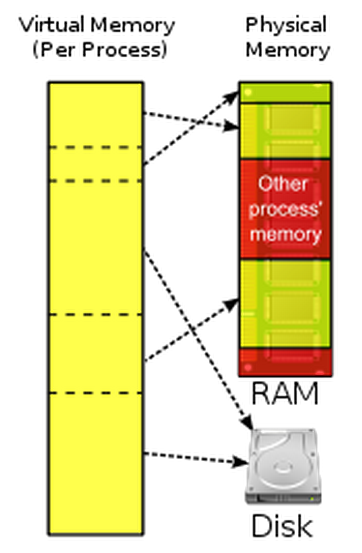
\includegraphics[width=0.3\linewidth]{bilder/virtualmemory.png}
\captionof{figure}{Wie virtueller Speicher funktioniert. Quelle: en.wikipedia.org, Virtual memory}
\end{center}

\noindent
In der Folge eine Beispielsausgabe aus unserem Messskript.

\begin{minipage}{\textwidth}
\begin{lstlisting}[language=bash,caption=Speicherdaten]{}
-----------------------
VmPeak:	 1086096 kB
VmSize:	 1036004 kB
VmLck:	       0 kB
VmHWM:	   15304 kB
VmRSS:	   15304 kB
VmData:	  988080 kB
VmStk:	     220 kB
VmExe:	      32 kB
VmLib:	   10960 kB
VmPTE:	     180 kB
-----------------------
\end{lstlisting}
\end{minipage}

\begin{table}[ht!]
\begin{tabular}[c]{|l|p{13cm}|} \hline
\textbf{Wert} & \textbf{Erklärung}\\
\hline
VmPeak & höchster Verbrauch von virtuellem Speicher den der Prozess seit dem Start jemals hatte\\
\hline
VmSize & aktueller Verbrauch von virtuellem Speicher. Darin ist auch VmData eingerechnet wodurch dieser Wert für die Messungen nicht weiter relevant ist (siehe VmData)\\
\hline
VmLck & Bei der virtuellen Speicherverwaltung wird der virtuelle Adressraum in Pages aufgeteilt. Aufgrund eines Fehlers kann es sein, dass eine solche Page gesperrt (locked) wird. Die Grösse des gesperrten Speichers würde, wenn vorhanden, hier angegeben.\\
\hline
VmHWM & HWM = high water mark, höchster Verbrauch von physikalischem Speicher den der Prozess seit dem Start jemals hatte\\
\hline
VmRSS & RSS = resident set size, aktueller Verbrauch von physikalischem Speicher\\
\hline
VmData & Daten auf denen das Programm ausgeführt wird. Sprich die JVM. Dieser Wert enthält auch Daten welche noch nicht in den Arbeitsspeicher geladen wurden weil sie nicht benötigt werden. Da für unsere Messungen nur die Daten im physikalischen Arbeitsspeicher interessant sind, ist dieser Wert für unsere Messungen daher irrelevant.\\
\hline
VmStk & Benötigte Ressourcen für die Ausführung. Dieser Wert ist eingerechnet in VmRSS.\\
\hline
VmExe & Der ausgeführte Programmcode, bzw. die als ausführbar markierten Pages. Dieser Wert ist eingerechnet in VmRSS.\\
\hline
VmLib & Shared Memory, Speicherbereich auf den auch andere Prozesse zugreifen können\\
\hline
VmPTE & Zwischen dem virtuellen und dem physikalischen Speicher befindet sich eine sog. Page Table welche den virtuellen Speicher dem physikalischen zuordnet  (z.B. virt. Adresse 0x01 befindet sich bei 0x0A im Arbeitsspeicher usw.). Die Grösse der Page Table ist in hier angegeben. \\
\hline							
\end{tabular}
\caption{Erklärung der gemessenen Speicherwerte}
\end{table}
\newpage
Zusammenfassend lässt sich sagen, dass für unsere Messungen lediglich der Wert VmRSS, welcher den tatsächlichen, physikalischen Speicherverbrauch abbildet, relevant ist. Dies weil die anderen Messwerte insofern verfälscht sind, dass sie teilweise gar nie in den Speicher geladen werden (VmPeak, VmSize, VmData) oder weil es für unsere Messungen nicht relevant ist wie gross die einzelnen Datensegmente (VmStk, VmExe) im Speicher sind.

\subsubsection{CPU}
In der Folge eine Beispielausgabe für die  Messung der CPU-Daten mit unserem Script. Neben dem ausführenden Benutzer und der Prozess-ID sind hier auch die momentane CPU-Auslastung und die vergangene Ausführzeit ersichtlich.

\begin{minipage}{\textwidth}
\begin{lstlisting}[language=bash,caption=Speicherdaten]{}
#
####26.02.2011 13:59:13####
#
USER       PID %CPU     TIME
root      7730  0.0 00:00:00
root      7730  0.0 00:00:00
root      7730 43.0 00:00:00
root      7730 65.0 00:00:00
root      7730 86.0 00:00:00
root      7730  112 00:00:01
root      7730  152 00:00:01
\end{lstlisting}
\end{minipage}

Bei Betrachtung dieser Daten fällt auf den ersten Blick auf, dass die CPU-Auslastung 100\% teilweise übersteigt. Da es sich beim Testsystem um ein Dual-Core System handelt, kann die CPU-Auslastung bis zu 200\% erreichen wenn beide Kerne zu 100\% ausgelastet sind. Aufgrund der heute von beinahe allen Betriebssystemen verwendeten SMP-Systemarchitektur, verwenden die Prozessoren unseres Testsystems einen gemeinsamen Adressraum um Aufgaben dynamisch verteilen zu können. Dies führt jedoch auch zu diesen, auf den ersten Blick verwirrenden, Messdaten. Da die gemessenen Daten aufgrund dessen jedoch keineswegs falsch sind, werden wir diese trotzdem für unsere Benchmarkes verwenden.

Die Spalte TIME gibt auf die Sekunde genau an, wie lange der Prozess bereits aktiv ist. Da wir die aktuellen Daten alle 0.2 Sekunden messen, ergeben sich fünf Zeilen pro Sekunde.

\subsubsection{Time}

Hier eine Beispielausgabe für die Messung der Zeit-Daten mit unserem Script. Erneut tauchen hier evtl. unbekannte Begriffe welche in der Folge kurz erklärt werden.

\begin{minipage}{\textwidth}
\begin{lstlisting}[language=bash,caption=Speicherdaten]{}
#
####26.02.2011 13:59:13####
#
Elapsed real time: 0:02.30
CPU usage: 99%
Total CPU-seconds in user mode: 2.38
Total CPU-seconds in kernel mode: 0.06
Name and arguments of the command: java -server -jar clojure/clojure.jar
\end{lstlisting}
\end{minipage}

\bigskip
\noindent
\underline{CPU-Modi:} Man unterscheidet zwischen zwei verschiedenen Betriebsmodi in denen die CPU Prozesse ausführt, es sind dies der Kernel- und der User-Modus.
\\\\
\underline{Kernel Mode:} Der ausgeführte Code hat unbeschränkten Zugang zur Hardware, kann jede Anweisung ausführen und jede Speicheradresse adressieren. Der Kernel Mode ist grundsätzlich für vertrauenswürdige Funktionen des Betriebssystems reserviert. Abstürze in diesem Mode können für das System verheerende Folgen haben.
\\\\
\underline{User Mode:} Der ausgeführte Code hat keine Möglichkeit direkt auf die Hardware zuzugreifen. Sollten solche Zugriffe nötig sein, müssen sie über Schnittstellen des Betriebssystems erfolgen. Durch die Einschränkungen entstehen bei Abstürzen keine Schäden am System.
\\\\
\underline{CPU-seconds:} Zeit in der die CPU tatsächlich mit der Ausführung des Prozesses beschäftigt war. Da durch das Betriebssystem immer auch andere Prozesse aktiv sind, dauert die Programmausführung in der Regel länger als die Anzahl CPU-Seconds die tatsächlich dafür aufgewendet wurden (CPU muss priorisieren). Aufgrund der Multicore Technologie ist es aber durchaus auch möglich, dass für eine Programmausführung mehr CPU-Seconds benötigt werden, als tatsächlich Zeit vergeht da die CPU-Seconds pro Kern gezählt werden.
\\
\begin{table}[h!]
\begin{tabular}[c]{|p{4cm}|p{11cm}|} \hline
\textbf{Wert} & \textbf{Erklärung}\\
\hline
Elapsed real time & Zeit die für die Programmausführung benötigt wurde\\
\hline
CPU usage & Durchschnittliche CPU-Auslastung während der Programmausführung\\
\hline
Total CPU-seconds in user mode & Im User-Mode verbrachte Zeit\\
\hline
Total CPU-seconds in kernel mode & Im Kernel-Mode verbrachte Zeit\\
\hline
Name and arguments of the command & Ausgeführtes Programm inkl. aller Parameter\\
\hline
\end{tabular}
\caption{Erklärung der gemessenen Zeitwerte}
\end{table}

\subsubsection{Methoden}
Für die Auswertung der Daten gehen wir wie folgt vor.
\begin{itemize}
\item Memory
\begin{itemize}
\item Vergleich des Verlaufes von VmRSS zwischen allen Programmiersprachen
\end{itemize}
\item CPU
\begin{itemize}
\item Vergleich des Verlaufes der CPU-Auslastung aller Programmiersprachen
\item Vergleich der durchschnittlichen CPU-Auslastung während der Ausführung
\end{itemize}
\item Zeit
\begin{itemize}
\item Vergleich der gesamten Ausführungszeit
\item Vergleich der benötigten CPU-seconds (Kernel- und User-Mode)
\end{itemize}
\end{itemize}
Alle Messresultate werden sowohl in tabellarischer wie auch in grafischer Form vorgelegt.
\section{Programmiersprachen und Implementierungen}

\subsection{Java}
\subsubsection{Beschreibung}

Java ist eine Programmiersprache, die ab 1992 von Sun Microsystems (oder
teilweise im Auftrag von Sun) entwickelt wurde. Java wurde zuerst f\"ur
eingebettete Systeme geschrieben. Heutzutage findet man Java Applikation in
vielen Anwendungsgebieten.
Java ist eine der meist verwendeten Programmiersprachen und wird auch
in vielen Universitäten gelehrt. 

\subsubsection{Code}

\lstinputlisting[language=Java]{../java/code.java}

\subsection{Scala}

\subsubsection{Beschreibung}

Die Entwicklung von Scala hat 2001 an der ETH Lausanne unter der Leitung von Martin
Odersky begonnen. Die Idee war eine Sprache zu designen, welche die
Konzepte von funktionalen und objektorientierten Sprachen in Synthese
verwendet. Zwar wurde Scala im akademischen Kontext entwickelt, findet
aber auch immer mehr Anwendungen im Business Bereich.

\subsubsection{Code}

\lstinputlisting[language=Scala]{../scala/code.scala}

\subsection{Clojure}
\subsubsection{Beschreibung}

Clojure ist eine dynamische Programmiersprache die 2007 von Rich Hicky
für die JVM geschrieben wurde. Im Vordergrund der Entwicklung standen
hohe Abstraktion, vor allem bei Concurency Programming, und eine gute
Integration ins Host System (JVM). Diese erlaubt die Wiederverwendung von
Java Code, Java Ecosystems (Webservers, Profilers, Debuggers...) und natürlich der VM.

\subsubsection{Code}

\lstinputlisting[langauge=Clojure]{../clojure/src/bt/binarytrees_me.clj}
\section{Ergebnisse}
Im diesem Kapitel werden die Messresultate der durchgeführten Messungen aufgezeigt. Hier ist zu beachten, dass es sich bei den Zeitangaben welche für die Memory- und CPU-Grafiken verwendet wurden, um Schätzungen handelt. Wir waren mit Hilfe unseres Scripts leider nicht in der Lage den genauen Zeitverlauf aufzuzeigen. Eventuelle Unregelmässigkeiten können daher nicht ausgeschlossen werden. Des weiteren beinhalten die in diesem Kapitel aufgezeigten Tabellen, aufgrund der grossen Datenmenge, nicht alle Messresultate. Die genaue Bedeutung der Werte wurde in den vorhergehenden Kapiteln bereits ausführlich behandelt, an dieser Stelle folgen daher keine Erklärungen mehr.

\subsection{Java}
\subsubsection{Allgemeine Daten}
Die folgende Tabelle beinhaltet einige allgemeine Messresultate zu Java. 
\begin{table}[h!]
\centering
\begin{tabular}{|p{6cm}|r|} \hline
Sprache & Java\\
\hline
Benötigte Zeit & 22.28s\\
\hline
Ø Speicherauslastung & 308557kB\\
\hline
Ø CPU-Auslastung & 109\%\\
\hline
Anz. CPU-Sekunden & 24.31s\\
\hline
davon im User-Mode & 23.74s\\
\hline
davon im Kernel-Mode & 0.57s\\
\hline
davon im User-Mode & 97.66\%\\
\hline
davon im Kernel-Mode & 2.34\%\\
\hline
\end{tabular}
\caption{Erklärung der gemessenen Zeitwerte Java}
\end{table}

\subsubsection{Memory}
Die nachfolgende Tabelle beinhaltet den Verlauf des physikalischen Speicherverbrauchs während der Ausführung des Java-Testprogrammes. Aufgrund der grossen Datenmenge haben wir uns auf einen Wert je zwei Sekunden Programmlaufzeit beschränkt. Die Grafik wurde unter Verwendung aller Messwerte erstellt, allfällige Spitzen sind darauf daher erkenntlich.
\begin{table}[h!]
\centering
\begin{tabular}{|r|r|} \hline
\textbf{Laufzeit [s]} & \textbf{Speicherverbrauch [kB]}\\
\hline
0 & 704\\
\hline
2 & 64888\\
\hline
4 & 398824\\
\hline
6 & 280544\\
\hline
8 & 287952\\
\hline
10 & 297992\\
\hline
12 & 314180\\
\hline
14 & 342300\\
\hline
16 & 394120\\
\hline
18 & 408484\\
\hline
20 & 419848\\
\hline
22 & 432032
\\
\hline
\end{tabular}
\caption{Wertetabelle Speicherverbrauch Java}
\end{table}
\begin{center}
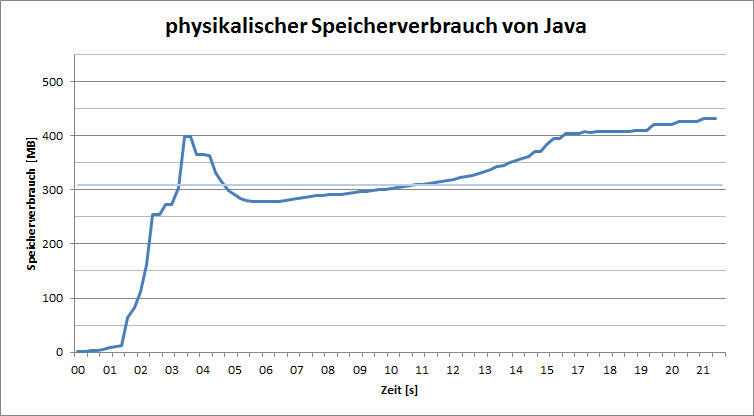
\includegraphics[width=\linewidth]{bilder/MemoryJava.png}
\captionof{figure}{Verlauf der Speicherauslastung Java}
\end{center}

\subsubsection{CPU}
Die nachfolgende Tabelle beinhaltet den Verlauf der CPU-Auslastung während der Ausführung des Java-Testprogrammes. Aufgrund der grossen Datenmenge haben wir uns auf einen Wert je zwei Sekunden Programmlaufzeit beschränkt. Die Grafik wurde unter Verwendung aller Messwerte erstellt, allfällige Spitzen sind darauf daher erkenntlich.
\begin{table}[h!]
\centering
\begin{tabular}{|r|r|} \hline
\textbf{Laufzeit [s]} & \textbf{CPU-Auslastung [\%]}\\
\hline
0 & 0\\
\hline
2 & 103\\
\hline
4 & 131\\
\hline
6 & 116\\
\hline
8 & 99.2\\
\hline
10 & 100\\
\hline
12 & 99.3\\
\hline
14 & 100\\
\hline
16 & 100\\
\hline
18 & 100\\
\hline
20 & 106\\
\hline
22 & 106
\\
\hline
\end{tabular}
\caption{Wertetabelle CPU-Auslastung Java}
\end{table}
\begin{center}
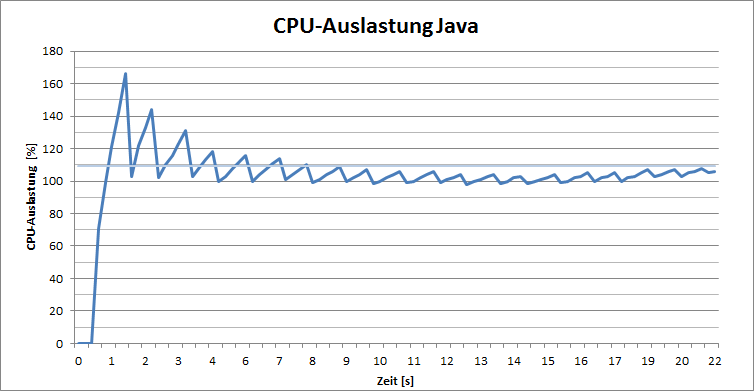
\includegraphics[width=\linewidth]{bilder/CPUJava.png}
\captionof{figure}{Verlauf CPU-Auslastung Java}
\end{center}


\subsection{Scala}
\subsubsection{Allgemeine Daten}
Die folgende Tabelle beinhaltet einige allgemeine Messresultate zu Scala. 
\begin{table}[h!]
\centering
\begin{tabular}{|p{6cm}|r|} \hline
Sprache & Scala\\
\hline
Benötigte Zeit & 22.37s\\
\hline
Ø Speicherauslastung & 297488kB\\
\hline
Ø CPU-Auslastung & 107\%\\
\hline
Anz. CPU-Sekunden & 24.03s\\
\hline
davon im User-Mode & 23.43s\\
\hline
davon im Kernel-Mode & 0.6s\\
\hline
davon im User-Mode & 97.50\%\\
\hline
davon im Kernel-Mode & 2.50\%\\
\hline
\end{tabular}
\caption{Erklärung der gemessenen Zeitwerte Scala}
\end{table}

\subsubsection{Memory}
Die nachfolgende Tabelle beinhaltet den Verlauf des physikalischen Speicherverbrauchs während der Ausführung des Scala-Testprogrammes. Aufgrund der grossen Datenmenge haben wir uns auf einen Wert je zwei Sekunden Programmlaufzeit beschränkt. Die Grafik wurde unter Verwendung aller Messwerte erstellt, allfällige Spitzen sind darauf daher erkenntlich.
\begin{table}[h!]
\centering
\begin{tabular}{|r|r|} \hline
\textbf{Laufzeit [s]} & \textbf{Speicherverbrauch [kB]}\\
\hline
0 & 548\\
\hline
2 & 145256\\
\hline
4 & 294424\\
\hline
6 & 228976\\
\hline
8 & 233204\\
\hline
10 & 245484\\
\hline
12 & 262084\\
\hline
14 & 293188\\
\hline
16 & 349612\\
\hline
18 & 443108\\
\hline
20 & 451776\\
\hline
22 & 493828\\
\hline
\end{tabular}
\caption{Wertetabelle Speicherverbrauch Scala}
\end{table}
\begin{center}
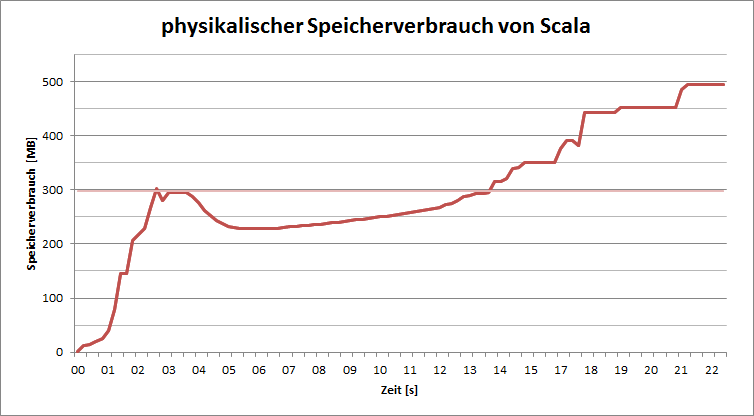
\includegraphics[width=\linewidth]{bilder/MemoryScala.png}
\captionof{figure}{Verlauf der Speicherauslastung Scala}
\end{center}

\subsubsection{CPU}
Die nachfolgende Tabelle beinhaltet den Verlauf der CPU-Auslastung während der Ausführung des Scala-Testprogrammes. Aufgrund der grossen Datenmenge haben wir uns auf einen Wert je zwei Sekunden Programmlaufzeit beschränkt. Die Grafik wurde unter Verwendung aller Messwerte erstellt, allfällige Spitzen sind darauf daher erkenntlich.
\begin{table}[h!]
\centering
\begin{tabular}{|r|r|} \hline
\textbf{Laufzeit [s]} & \textbf{CPU-Auslastung [\%]}\\
\hline
0 & 0\\
\hline
2 & 105\\
\hline
4 & 103\\
\hline
6 & 100\\
\hline
8 & 101\\
\hline
10 & 100\\
\hline
12 & 100\\
\hline
14 & 100\\
\hline
16 & 100\\
\hline
18 & 99.3\\
\hline
20 & 100\\
\hline
22 & 105\\
\hline
\end{tabular}
\caption{Wertetabelle CPU-Auslastung Scala}
\end{table}
\begin{center}
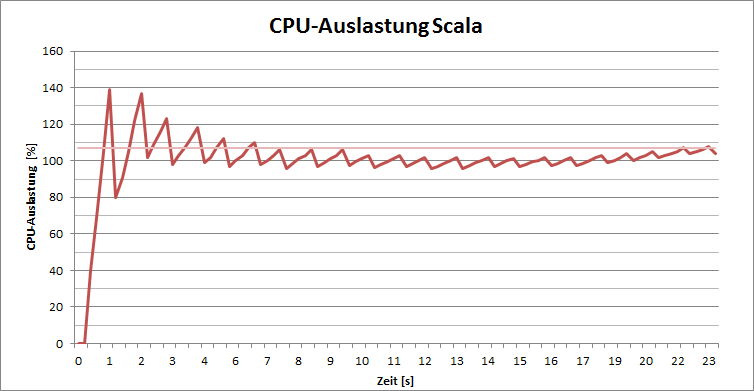
\includegraphics[width=\linewidth]{bilder/CPUScala.png}
\captionof{figure}{Verlauf CPU-Auslastung Scala}
\end{center}

\subsection{Clojure}
\subsubsection{Allgemeine Daten}
Die folgende Tabelle beinhaltet einige allgemeine Messresultate zu Clojure. 
\begin{table}[h!]
\centering
\begin{tabular}{|p{6cm}|r|} \hline
Sprache & Clojure\\
\hline
Benötigte Zeit & 59.92s\\
\hline
Ø Speicherauslastung & 527627kB\\
\hline
Ø CPU-Auslastung & 112\%\\
\hline
Anz. CPU-Sekunden & 67.52s\\
\hline
davon im User-Mode & 66.66s\\
\hline
davon im Kernel-Mode & 0.86s\\
\hline
davon im User-Mode & 98.73\%\\
\hline
davon im Kernel-Mode & 1.27\%\\
\hline
\end{tabular}
\caption{Erklärung der gemessenen Zeitwerte Clojure}
\end{table}

\subsubsection{Memory}
Die nachfolgende Tabelle beinhaltet den Verlauf des physikalischen Speicherverbrauchs während der Ausführung des Clojure-Testprogrammes. Aufgrund der grossen Datenmenge haben wir uns auf einen Wert je fünf Sekunden Programmlaufzeit beschränkt. Die Grafik wurde unter Verwendung aller Messwerte erstellt, allfällige Spitzen sind darauf daher erkenntlich.
\begin{table}[h!]
\centering
\begin{tabular}{|r|r|} \hline
\textbf{Laufzeit [s]} & \textbf{Speicherverbrauch [kB]}\\
\hline
0 & 8660\\
\hline
5 & 432428\\
\hline
10 & 491620\\
\hline
15 & 499872\\
\hline
20 & 506064\\
\hline
25 & 507408\\
\hline
30 & 514368\\
\hline
35 & 546104\\
\hline
40 & 574592\\
\hline
45 & 619920\\
\hline
50 & 661224\\
\hline
55 & 661296\\
\hline
59.8 & 666592\\
\hline
\end{tabular}
\caption{Wertetabelle Speicherverbrauch Clojure}
\end{table}
\begin{center}
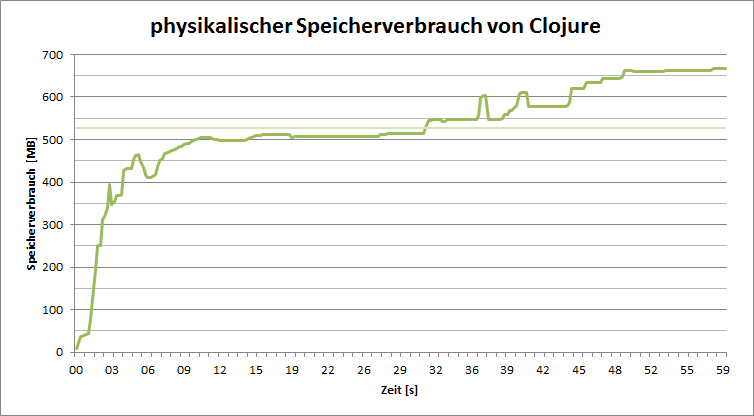
\includegraphics[width=\linewidth]{bilder/MemoryClojure.png}
\captionof{figure}{Verlauf der Speicherauslastung Clojure}
\end{center}

\subsubsection{CPU}
Die nachfolgende Tabelle beinhaltet den Verlauf der CPU-Auslastung während der Ausführung des Clojure-Testprogrammes. Aufgrund der grossen Datenmenge haben wir uns auf einen Wert je fünf Sekunden Programmlaufzeit beschränkt. Die Grafik wurde unter Verwendung aller Messwerte erstellt, allfällige Spitzen sind darauf daher erkenntlich.
\begin{table}[h!]
\centering
\begin{tabular}{|r|r|} \hline
\textbf{Laufzeit [s]} & \textbf{CPU-Auslastung [\%]}\\
\hline
0 & 0\\
\hline
5 & 150\\
\hline
10 & 125\\
\hline
15 & 117\\
\hline
20 & 115\\
\hline
25 & 111\\
\hline
30 & 110\\
\hline
35 & 106\\
\hline
40 & 104\\
\hline
45 & 108\\
\hline
50 & 112\\
\hline
55 & 109\\
\hline
59.8 & 109\\
\hline
\end{tabular}
\caption{Wertetabelle CPU-Auslastung Clojure}
\end{table}
\begin{center}
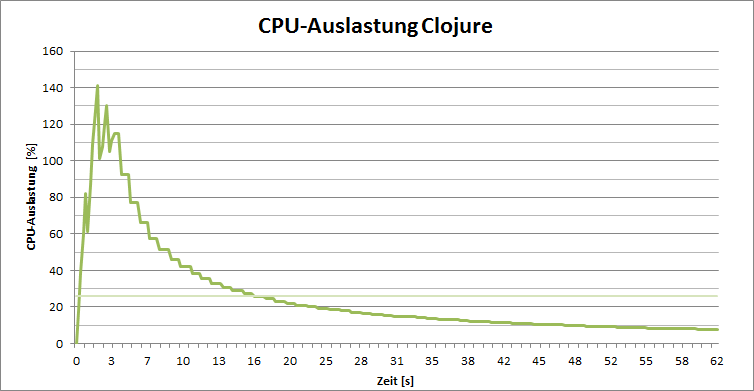
\includegraphics[width=\linewidth]{bilder/CPUClojure.png}
\captionof{figure}{Verlauf CPU-Auslastung Clojure}
\end{center}

\section{Diskussion}
\subsection{Vergleich der Resultate}
\subsubsection{Zeitspezifische Daten}
In diesem Unterkapitel vergleichen wir die jene Messdaten, welche die Zeit betreffen, d.h. die realen Ausführungszeiten und die benötigten CPU-Sekunden. Genau diese Werte wurden in Abbildung Nr. 8 grafisch dargestellt. Es ist deutlich ersichtlich wie Java und Scala sich ein Kopf-an-Kopf-Rennen liefern während Clojure mit einer ca. dreimal so hohen Ausführungszeit weit abgeschlagen ist. Das gleiche Bild zeigt sich bei den CPU-Sekunden, wo die Differenz noch grösser ist. Vergleicht man die Messungen von Java und Scala etwas genauer, so hat Scala bei nahezu gleicher Ausführungszeit etwas weniger CPU-Sekunden benötigt. Scala könnte daher als knapper 'Sieger' dieser Messung bezeichnet werden.
\begin{table}[h!]
\centering
\begin{tabular}{|p{6cm}|r|r|r|} \hline
Sprache & Java & Scala & Clojure \\
\hline
Benötigte Zeit & 22.28s & 22.37s & 59.62s\\
\hline
Anz. CPU-Sekunden & 24.31s & 24.03s & 67.52s\\
\hline
davon im User-Mode & 23.74s & 23.42s & 66.66s\\
\hline
davon im Kernel-Mode & 0.57s & 0.6s & 0.86s\\
\hline
davon im User-Mode & 97.66\% & 97.50\% & 98.73\%\\
\hline
davon im Kernel-Mode & 2.34\% & 2.50\% & 1.27\%\\
\hline
\end{tabular}
\caption{Erklärung der gemessenen Zeitwerte Clojure}
\end{table}
\begin{center}
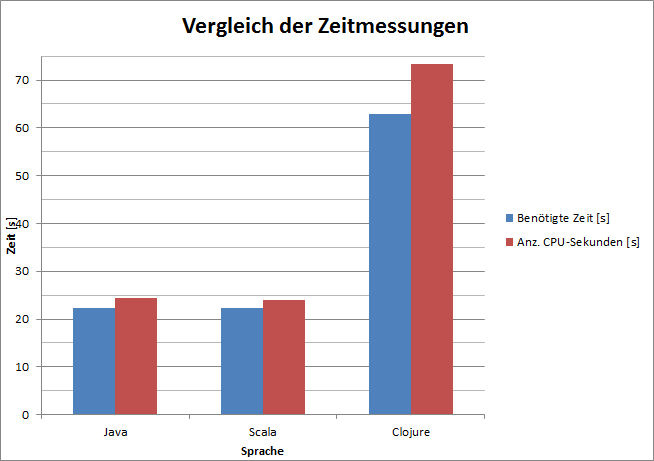
\includegraphics[width=\linewidth]{bilder/TimeAll.png}
\captionof{figure}{Vergleich der Zeitmessungen}
\end{center}
Abbildung Nr. 9 zeigt den prozentualen Anteil an CPU-Sekunden auf, welcher im Kernel-Mode verbracht werden musste. Hier sieht das Bild schon wieder ganz anders aus. Clojure verbrachte rund ein Prozent weniger Ausführungszeit im Kernel-Mode als die anderen beiden Sprachen. Scala liegt mit einem Anteil von 2.5\% auf dem letzten Platz. Es muss hier jedoch angemerkt werden, dass es unklar ist wann genau die CPU diese Zeit benötigt hat. Sollte sich dies auf den Programmstart beschränken, wird der Prozentsatz der CPU-Sekunden im Kernel-Mode bereits durch die lange Ausführungszeit des Clojure-Programms hinuntergezogen. Leider lässt sich dies nur sehr schlecht prüfen.
\begin{center}
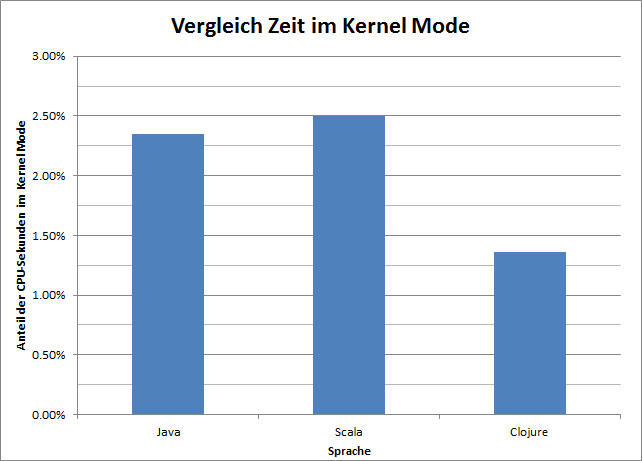
\includegraphics[width=\linewidth]{bilder/KernelModeAll.png}
\captionof{figure}{Vergleich des Anteils an CPU-Sekunden, welche im Kernel Mode verbracht wurden}
\end{center}

\subsubsection{Memory}
Die folgende Grafik vergleicht die Speicherdaten aller Sprachen. Clojure hat den anderen Sprachen gegenüber einen deutlich höheren Speicherverbrauch. Jedoch verläuft auch der Verbrauch von Clojure  ähnlich wie derjenige der anderen Sprachen. Kurz nach dem Programmstart steigt der Speicherverbrauch enorm an, bleibt dann eine Weile auf ungefähr gleichbleibendem Niveau, bevor er vor dem Programmende erneut stark ansteigt. Der Speicherverbrauch von Java und Scala entwickelt sich sehr ähnlich, jedoch ist der Arbeitsspeicherverbrauch von Scala etwas tiefer als jener von Java. Erst kurz vor Programmende steigt der Verbrauch von Scala nochmal stark an und übersteigt jenen von Java. Dementspreichend ist der durchschnittliche Speicherverbrauch von Clojure mit einer Differenz von ungefähr 200MB mit Abstand der höchste, gefolgt von Java und Scala.

\bigskip
\noindent
Ein Hinweis zur Tabelle: Aufgrund der grossen Datenmenge enthält die Wertetabelle jeweils nur einen Wert je Sekunde Ausführungszeit. Des Weiteren ist die Spalte für Clojure nicht vollständig, da ab Sekunde 23 kein Vergleich mehr mit den anderen Sprachen möglich ist.


\begin{center}
\begin{tabular}{|r|r|r|r|} \hline
\textbf{Zeit [s]} & \textbf{Java [kB]} & \textbf{Scala [kB]} & \textbf{Clojure [kB]}\\
\hline
0 & 704 & 548 & 8660\\
\hline
1 & 4076 & 24504 & 41604\\
\hline
2 & 64888 & 145256 & 194040\\
\hline
3 & 254820 & 301740 & 340340\\
\hline
4 & 398824 & 294424 & 369344\\
\hline
5 & 315296 & 243544 & 432428\\
\hline
6 & 280544 & 228976 & 449356\\
\hline
7 & 278380 & 228492 & 412020\\
\hline
8 & 287952 & 233204 & 468172\\
\hline
9 & 292080 & 239428 & 479828\\
\hline
10 & 297992 & 245484 & 491620\\
\hline
11 & 305280 & 252520 & 504148\\
\hline
12 & 314180 & 262084 & 503488\\
\hline
13 & 324204 & 275336 & 497592\\
\hline
14 & 342300 & 293188 & 497532\\
\hline
15 & 357680 & 320268 & 499872\\
\hline
16 & 394120 & 349612 & 510348\\
\hline
17 & 404572 & 376812 & 511356\\
\hline
18 & 408484 & 443108 & 511824\\
\hline
19 & 408484 & 443236 & 512052\\
\hline
20 & 419848 & 451776 & 506064\\
\hline
21 & 425884 & 451780 & 506420\\
\hline
22 & 432032 & 493828 & 506292\\
\hline
... & - & - & ...\\
\hline
Ø & 308557 & 297488 & 527627\\
\hline
\end{tabular}
\captionof{table}{Vergleich der gemessenen Speicherdaten}

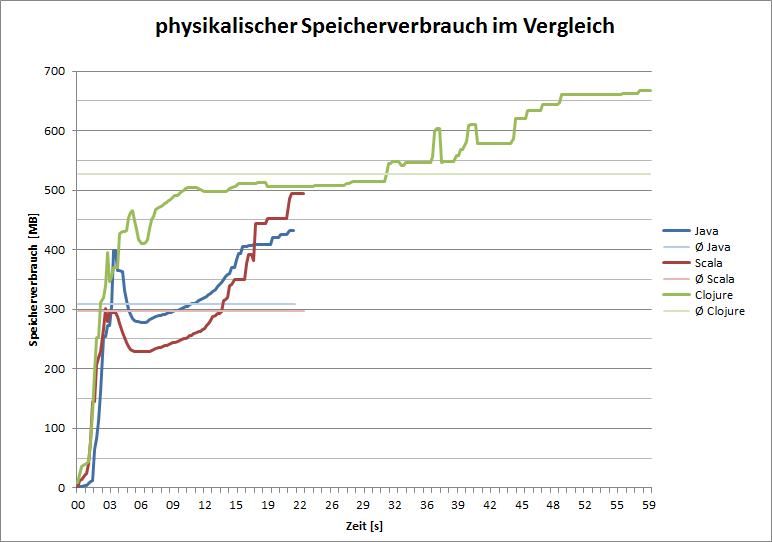
\includegraphics[width=\linewidth]{bilder/MemoryAll.png}
\captionof{figure}{Vergleich des Speicherverbrauchs}
\end{center}
\subsubsection{CPU}
Die folgende Grafik zeigt die CPU-Auslastung während der Programmausführung an. Anfangs steigt die CPU-Auslastung bei allen Sprachen ungefähr gleich stark an. Während sich Java und Clojure anschliessend während der ganzen Programmausführung in einem Bereich von ca. 100\% bewegen, ist die CPU-Auslastung beim Clojure-Programm vor allem anfangs deutlich höher. Nach ungefähr 25 Sekunden pendelt sich das Clojure-Programm bei ca. 110\% ein. Beim genaueren Vergleich von Java und Scala fällt auf, dass die CPU-Auslastung bei Java stets minimal höher ist als bei Scala. Auch bei dieser Messung ist der Ressourcenverbrauch von Clojure am höchsten.

\bigskip
\noindent
Ein Hinweis zur Tabelle: Aufgrund der grossen Datenmenge enthält die Wertetabelle jeweils nur einen Wert je Sekunde Ausführungszeit. Des Weiteren ist die Spalte für Clojure nicht vollständig, da ab Sekunde 23 kein Vergleich mehr mit den anderen Sprachen möglich ist.

\begin{center}
\begin{tabular}{|r|r|r|r|} \hline
\textbf{Zeit [s]} & \textbf{Java [\%]} & \textbf{Scala [\%]} & \textbf{Clojure [\%]}\\
\hline
0 & 0 & 0 & 0\\
\hline
1 & 99 & 105 & 0\\
\hline
2 & 103 & 105 & 200\\
\hline
3 & 144 & 102 & 142\\
\hline
4 & 131 & 103 & 153\\
\hline
5 & 99.8 & 102 & 150\\
\hline
6 & 116 & 100 & 147\\
\hline
7 & 114 & 100 & 143\\
\hline
8 & 99.2 & 101 & 141\\
\hline
9 & 100 & 101 & 125\\
\hline
10 & 100 & 101 & 125\\
\hline
11 & 100 & 101 & 126\\
\hline
12 & 99.3 & 100 & 123\\
\hline
13 & 99.6 & 100 & 121\\
\hline
14 & 100 & 100 & 120\\
\hline
15 & 99.7 & 100 & 117\\
\hline
16 & 100 & 100 & 117\\
\hline
17 & 100 & 100 & 115\\
\hline
18 & 100 & 100 & 113\\
\hline
19 & 107 & 100 & 117\\
\hline
20 & 103 & 103 & 115\\
\hline
21 & 105 & 105 & 112\\
\hline
22 & 106 & 105 & 111\\
\hline
... & - & - & ...\\
\hline
Ø & 109 & 107 & 112\\
\hline
\end{tabular}
\captionof{table}{Vergleich der gemessenen CPU-Auslastungen}

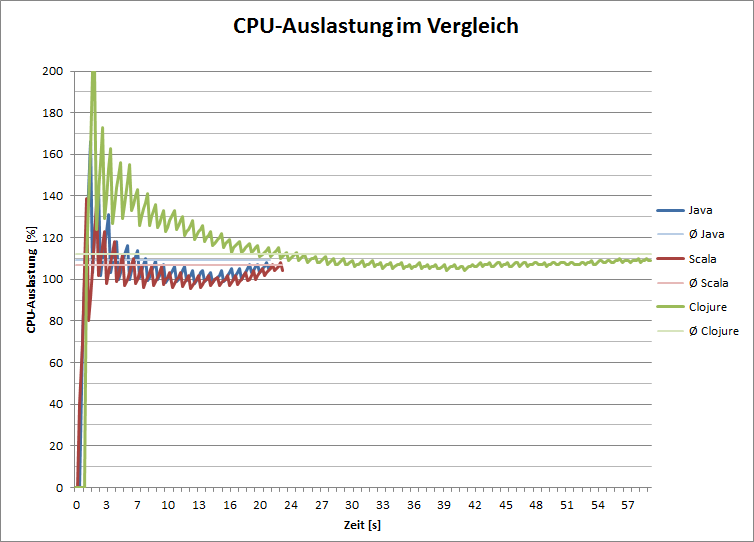
\includegraphics[width=.9\linewidth]{bilder/CPUAll.png}
\captionof{figure}{Vergleich der CPU-Auslastung}
\bigskip
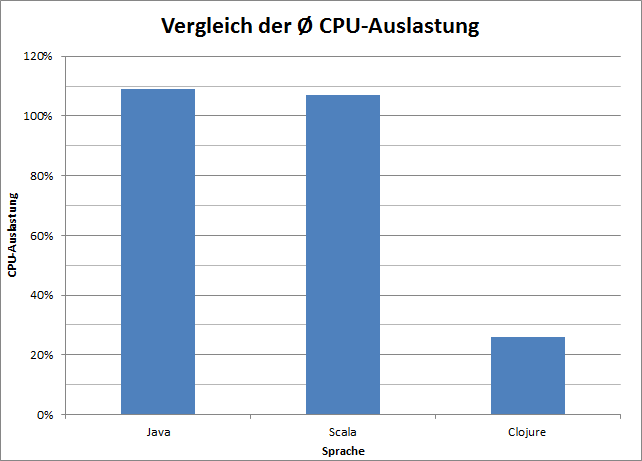
\includegraphics[width=.9\linewidth]{bilder/AverageCPUAll.png}
\captionof{figure}{Vergleich der durchschnittlichen CPU-Auslastung}
\end{center}

\subsection{Schlussfolgerung}
Die Messresultate entsprechen weitgehend den Erwartungen. Wie es sich auch schon bei anderen Benchmarkes gezeigt hat, sind die Messresultate von Java und Scala sehr ähnlich. Etwas überraschend war lediglich die leicht tiefere Systembelastung von Scala gegenüber Java. Dies bei einer Ausführungszeit welche mit einer Differenz von 0.1 Sekunden beinahe identisch mit derjenigen von Java ist. Clojure ist, wie bei einer so jungen Sprache auch nicht anders zu erwarten, verglichen mit den anderen Sprachen weit abgeschlagen. Zwar ist lag die Belastung von CPU und Memory während der Ausführung stets tiefer als bei den anderen Sprachen, mit einer Zeit von über einer Minute dauerte die Ausführung jedoch ungefähr drei Mal so lange. Da heutige Systeme sehr performant sind und über ausreichend Arbeitsspeicher und Rechenleistung verfügen, wäre eine bessere Nutzung der Ressourcen wünschenswerter gewesen wenn sich dadurch die Ausführzeit verringert hätte. Schliesslich sind die zusätzlichen Ressourcen ja dazu da um genutzt zu werden und damit das System zu verschnellern.
Zusammenfassend lässt sich sagen, dass Java und Scala aufgrund der Messresultate auch für Grossprojekte sehr geeignet sind. Diese gehören, wie sich aus externen Tests schliessen lässt, mitunter zu den schnellsten Programmiersprachen überhaupt. Clojure hingegen kann (noch) nicht mit diesen Programmiersprachen mithalten. Es ist daher vor allem bei grösseren Projekte ratsam zu prüfen, ob die von Clojure erbrachte Geschwindigkeit für das Projekt ausreichend ist.

\section{Abk\"urzungsverzeichnis}
\begin{tabbing}
\hspace*{2cm}\=\kill
\textbf{CPU} \>Central Processing Unit\\
\textbf{HWM} \>High Water Mark\\
\textbf{IL} \>Intermediate Language\\
\textbf{JVM} \>Java Virtual Machine\\
\textbf{PID} \>Process Identifier\\
\textbf{procfs}\>Process Filesystem\\
\textbf{PS} \>Process Status\\
\textbf{PTE} \>Page Table Entry\\
\textbf{RAM} \>Random Access Memory\\
\textbf{RSS} \>Resident Set Size\\
\textbf{SED} \>Stream Editor\\
\textbf{SMP} \>Symmetric Multiprocessing\\
\textbf{VM} \>Virtual Machine\\
\end{tabbing}


\section{Glossar}
\renewcommand{\arraystretch}{1.4}
\begin{tabularx}{\linewidth}{p{6.5cm}X}
\textbf{Arbeitsspeicher}&auch Hauptspeicher, dient zum kurzzeitigen Speichern von Daten und ist massiv schneller als Festplatten\\
\textbf{Befehlssatz}&Eine Menge von Befehlen, welche in Maschinensprache vorliegt\\
\textbf{Bytecode}&Ein Befehlssatz für eine VM.\\
\textbf{CPU-Modi}&siehe Kapitel 4.5.3 (Time)\\
\textbf{CPU-second}&siehe Kapitel 4.5.3 (Time)\\
\textbf{Debian}&Ein frei erhältliches Client-Betriebssystem welches auf einem Linux-Kernel basiert\\
\textbf{Hardware}&mechanische und elektronische Teile eines beliebigen Systems, dazu gehören auch Computer\\
\textbf{Java Bytecode}&Der Bytecode für Java bzw. für die JVM\\
\textbf{Java Virtual Machine}&Die Implementierung einer VM, welche darauf ausgelegt ist Java Bytecode auszuführen.\\
\textbf{Kernel Mode}&siehe Kapitel 4.5.3 (Time)\\
\textbf{Kompilierung}&Übersetzung von Quellcode einer Programmiersprache in Maschinensprache\\
\textbf{Maschinensprache}&Befehle, die der Prozessor ohne Kompilierung ausführen kann\\
\textbf{Open-Source}&Software deren Quellcode öffentlich zugänglich ist\\
\textbf{Page}&eine Einheit in die der Arbeitsspeicher unterteilt wird, es handelt sich um die kleinste Speichereinheit, in der Reservationen durchgeführt werden\\
\textbf{Parallelisierung}&Aufteilung eines Programms in mehrere Teile, die gleichzeitig ausgeführt werden können. Das Programm wird dadurch multiprozessorfähig\\
\textbf{Parameter}&ein Wert der einem Programm oder Script mitgegeben wird\\
\end{tabularx}
\newpage
\noindent
\begin{tabularx}{\linewidth}{p{6.5cm}X}
\textbf{Performance-Monitoring-Tool}&Programm, welches die Leistungsdaten eines Computers oder Prozesses überwacht\\
\textbf{Proc}&ein virtuelles Dateisystem welches System- und Prozessinformationen anzeigt\\
\textbf{Script}&ein in einer Scriptsprache geschriebenes Programm\\
\textbf{Scriptsprache}&Programmiersprache, welche sich speziell für kleine Programme eignet\\
\textbf{User Mode}&siehe Kapitel 4.5.3 (Time)\\
\textbf{Virtual Machine}&Eine Programm, welches einen physikalischen Computer simuliert. Sie erhält als Input eine beliebige Sprache und führt
diese auf der darunterliegenden Sprache aus.\\
\textbf{Virtual Memory}&siehe Kapitel 4.5.1 (Memory)\\
\end{tabularx}
\section{Literaturverzeichnis}
\noindent
\begin{tabularx}{\linewidth}{@{$\bullet$  }v{15cm}@{}}
Bird, Tim (2009): Runtime Memory Measurement
http://elinux.org/Runtime\_Memory\_Measurement (26.02.2011)\tabularnewline[3pt]
Feiner, Tom (2009): Peak memory usage of a process
http://serverfault.com/questions/11550/peak-memory-usage-of-a-process (26.02.2011)\tabularnewline[3pt]
Fulgham, Brent (2011): The Computer Language Benchmarks Game.
http://shootout.alioth.debian.org/ (26.02.2011)\tabularnewline[3pt]
Gmane.org, Benutzer: shivaligupta (2006): Regarding /proc/<pid>/status
http://article.gmane.org/gmane.linux.kernel.kernelnewbies/15454/match= (26.02.2011)\tabularnewline[3pt]
Kerrisk, Michael (2010): proc - process information pseudo-file system.
bhttp://www.kernel.org/doc/man-pages/online/pages/man5/proc.5.html (26.02.2011)\tabularnewline[3pt]
Mackintosh, David (2010): A definition for a CPU second?
http://serverfault.com/questions/138703/a-definition-for-a-cpu-second (26.02.2011)\tabularnewline[3pt]
McGrath, Roland (2007): Locking Pages
http://www.gnu.org/s/libc/manual/html\_node/Locking-Pages.html#Locking-Pages (26.02.2011)\tabularnewline[3pt]
Santosa, Mulyadi (2006): When Linux Runs Out of Memory.
http://linuxdevcenter.com/pub/a/linux/2006/11/30/linux-out-of-memory.html (26.02.2011)\tabularnewline[3pt]
Turakhia, Bhavin (2010): Understanding and optimizing Memory utilization.
http://careers.directi.com/display/tu/Understanding+and+optimizing+Memory+ utilization (26.02.2011)\tabularnewline[3pt]
University of Alberta (2010): Understanding Memory
http://www.ualberta.ca/CNS/RESEARCH/LinuxClusters/mem.html (26.02.2011)\tabularnewline[3pt]
Unix.com, Benutzer: sysgate (2008): top command + \%CPU usage exceeds 100\%?
http://www.unix.com/unix-dummies-questions-answers/92541-top-command-cpu-usage-exceeds-100-a.html (26.02.2011)\tabularnewline[3pt]
\end{tabularx}
\newpage
\noindent
\begin{tabularx}{\linewidth}{@{$\bullet$  }v{15cm}@{}}
Wikipedia, Benutzer: Guy Harris (2011): Page table
http://en.wikipedia.org/wiki/Page\_table (26.02.2011)\tabularnewline[3pt]
Wikipedia, Benutzer: MetaEntropy (2010): Code segment.
http://en.wikipedia.org/wiki/Code\_segment (26.02.2011)\tabularnewline[3pt]
Wikipedia, Benutzer: Mindmatrix (2011): Stack (data structure)
http://en.wikipedia.org/wiki/Stack\_(data\_structure) (26.02.2011)\tabularnewline[3pt]
Wikipedia, Benutzer: Nat682 (2011): Memory segmentation.
http://en.wikipedia.org/wiki/Segmentation\_(memory) (26.02.2011)\tabularnewline[3pt]
Wikipedia, Benutzer: Rich Farmbrough (2009): Resident set size.
http://en.wikipedia.org/wiki/Resident\_set\_size (26.02.2011)\tabularnewline[3pt]
Wikipedia, unbekannter Autor (2011): Data segment.
http://en.wikipedia.org/wiki/Data\_segment (26.02.2011)\tabularnewline[3pt]
Wikipedia, unbekannter Autor (2011): Virtual memory.
http://en.wikipedia.org/wiki/Virtual\_memory (26.02.2011)\tabularnewline[3pt]
\end{tabularx}

\section{Anhang}

Wir erklären hiermit, dass wir die vorliegende interdisziplinäre Projektarbeit eigenständig und ohne unerlaubte fremde Hilfe erstellt haben und dass alle Quellen, Hilfsmittel und Internetseiten wahrheitsgetreu verwendet wurden und belegt sind.

\begin{tabbing}
\hspace*{5cm}\=\hspace*{5cm}\=\kill
Ort: \>Datum: \>Unterschrift:\\
\end{tabbing}

\end{document}
